\section{Sobre o Autor}

\begin{figure}[h]
  \centering

  \begin{minipage}{0.28\textwidth}
    \centering
    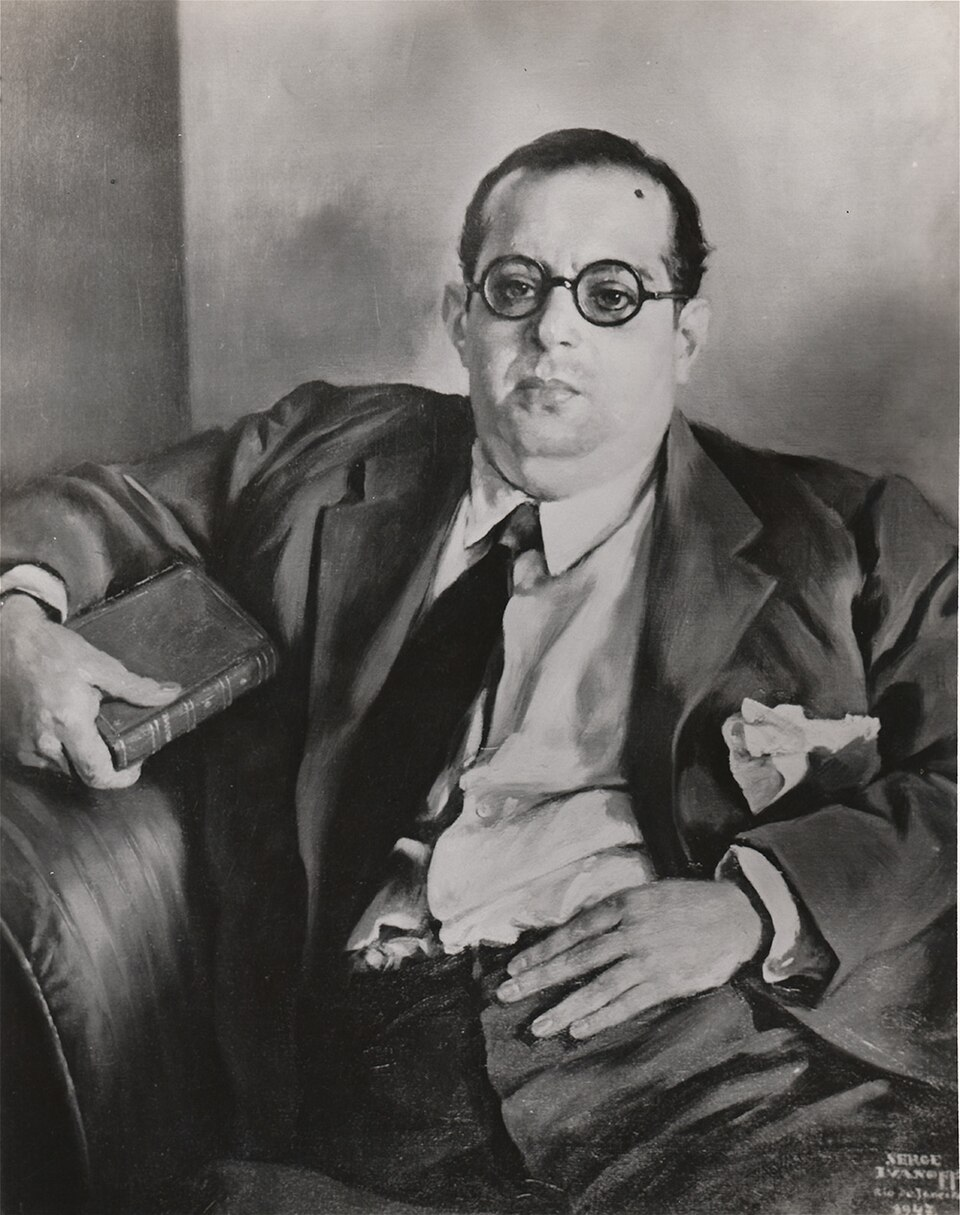
\includegraphics[width=\linewidth]{./fig/Augusto-Frederico-Schmidt.jpg}

    \vspace{0.5em}
    \footnotesize
    Augusto Frederico Schmidt\\
    (1906--1965)
  \end{minipage}
  \hfill
  \begin{minipage}{0.7\textwidth}
    Augusto Frederico Schmidt (Rio de Janeiro, 18 de abril de 1906 -- Rio
    de Janeiro, 8 de fevereiro de 1965) foi poeta, editor, empresário,
    diplomata e homem público brasileiro. Filho de um imigrante judeu
    asquenaze alemão e neto do Visconde de Schmidt, iniciou sua trajetória
    no mercado editorial após atuar na Livraria Católica e, em 1930, fundou
    a Livraria Schmidt Editora.\\

    À frente da editora, publicou as primeiras obras de autores que se
    tornariam fundamentais para a literatura brasileira, entre eles Gilberto
    Freyre, Graciliano Ramos, Rachel de Queiroz, Jorge Amado, Vinicius de
    Moraes, Lúcio Cardoso e Octávio de Faria. A Livraria Schmidt tornou-se um
    dos principais centros da vida intelectual carioca na década de 1930,
    servindo como ponto de encontro do chamado \textit{Círculo Católico},
    grupo informal que reunia escritores, jornalistas e pensadores ligados ao
    renascimento do pensamento católico no Brasil na época. \\

    Paralelamente à atividade literária, desenvolveu uma carreira de
    sucesso como empresário, atuando nos setores editorial, de seguros,
    mineração, aviação e varejo. Também exerceu funções diplomáticas e foi
    assessor especial do presidente Juscelino Kubitschek, sendo
    tradicionalmente associado à criação do slogan ``50 anos em 5''.
    Faleceu no Rio de Janeiro em 1965, deixando uma obra poética que
    permanece entre as mais singulares da literatura brasileira do século
    XX.
  \end{minipage}
\end{figure}

\section{Por que este poema?}

A escolha de \textit{Era Um Grande Pássaro} parte da convicção de que Augusto
Frederico Schmidt ocupa um lugar muito mais elevado na literatura brasileira do
que aquele que lhe é normalmente atribuído. Figura central da vida intelectual
das décadas de 1930 e 1940, editor responsável pela publicação de alguns dos
mais importantes escritores brasileiros e autor de uma obra poética singular,
Schmidt acabou gradualmente relegado a uma posição secundária na historiografia
literária.

Seu relativo esquecimento decorre, em grande parte, da combinação de fatores
estéticos e ideológicos. Enquanto a crítica passou a privilegiar uma poesia
cada vez mais identificada com o experimentalismo modernista, Schmidt manteve
uma escrita marcada pela espiritualidade, pelo simbolismo, pela musicalidade e
pela permanência de formas clássicas. Sua declarada identidade católica e sua
participação na articulação inicial do integralismo brasileiro também
contribuíram para que sua obra fosse frequentemente lida à luz de suas posições
políticas, em detrimento de seus méritos literários.

Essa tensão já era perceptível em sua própria época. A conhecida crítica de
Mário de Andrade ilustra o desencontro entre dois projetos estéticos e
intelectuais distintos. Como observa Leandro Garcia Rodrigues, enquanto Mário
propunha uma constante renovação da linguagem literária, Schmidt permanecia
ligado à tradição poética e a uma visão profundamente religiosa da literatura,
diferenças agravadas pelas divergências políticas e religiosas entre ambos
\cite{rodrigues2018}. A influência exercida por Mário sobre a crítica
universitária contribuiu para consolidar uma leitura pouco favorável da obra de
Schmidt ao longo da segunda metade do século XX.

Apesar disso, Schmidt desfrutava de enorme prestígio entre muitos de seus
contemporâneos. Manuel Bandeira, por exemplo, prestou-lhe homenagem no poema
\textit{À Maneira de Augusto Frederico Schmidt}
\cite[p.~111]{bandeira1955mafua}. O fato de um dos principais poetas
brasileiros do século XX dedicar um poema a Schmidt constitui um testemunho
eloquente do respeito que sua obra despertava entre seus pares e evidencia que
sua recepção esteve longe de ser unanimemente
desfavorável.

Este estudo procura, portanto, revisitar um poeta cuja obra permanece
insuficientemente lida. \textit{Era Um Grande Pássaro} reúne algumas das
qualidades mais características de Schmidt: a intensidade imagética, a
musicalidade dos versos, a dimensão simbólica e a profunda reflexão sobre a
morte, o mistério e a transcendência. É um poema que evidencia por que sua
produção merece voltar ao centro das discussões sobre a poesia brasileira do
século XX.
